\documentclass{article}
\usepackage[utf8]{inputenc}
\usepackage{amsmath}
\usepackage{amsfonts}
\usepackage{graphicx}

\newcommand\tr{\mathsf{T}}

\begin{document}

\section*{Polar Decomposition of Matrices}
In this exercise we look at one more decomposition of matrices called the \textbf{polar decomposition}.

\begin{figure}[!hbt]
    \centering
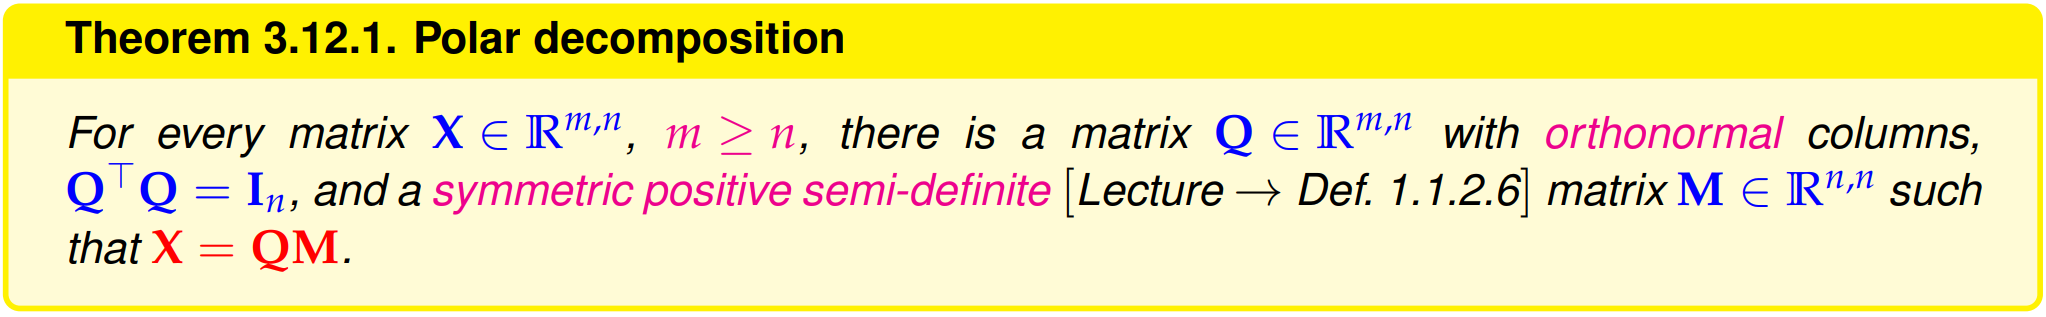
\includegraphics[width=1.0\linewidth]{PolarDecomposition.png}
\end{figure}

\subsection*{3-12.a}
We are tasked with stating a proof for Theorem 3.12.1. Let $\mathbf{X}\in \mathbb{R}^{m,n}$ be some matrix, we know that there exists a SVD for $\mathbf{X}$, with
\begin{equation*}
    \mathbf{X} = \mathbf{U}\mathbf{\Sigma}\mathbf{V}^{\mathsf{T}}
\end{equation*}
we know that the matrix $\mathbf{\Sigma}$ is diagonal and that both $\mathbf{U}$ and $\mathbf{U}$ have orthonormal columns. In the case that $\mathbf{X}\in \mathbb{R}^{m,n}$ The theorem also tells us that $m \geq n$, in that case we have that $\mathbf{U}\in \mathbb{R}^{m,n}$ $\Sigma \in \mathbb{R}^{n,n}$ and $\mathbf{V}\in \mathbb{R}^{n,n}$. We then in this case have that $\mathbf{U}$ has orthonormal columns (is not orthogonal though) and $\mathbf{V}$ is orthogonal (and thus also has orthonormal columns). This means that we have
\begin{align*}
    \mathbf{U}^{\mathsf{T}}\mathbf{U} &= \mathbf{I} \\
    \mathbf{V}^{\mathsf{T}}\mathbf{V}& = \mathbf{V}\mathbf{V}^{\mathsf{T}} = \mathbf{I}
\end{align*}
We can use this to see that
\begin{equation*}
    \mathbf{X} = \mathbf{U}\mathbf{\Sigma}\mathbf{V}^{\mathsf{T}} = \mathbf{U}\mathbf{I}\mathbf{\Sigma}\mathbf{V}^{\mathsf{T}} = \mathbf{U}\mathbf{V}^{\mathsf{T}}\mathbf{V}\mathbf{\Sigma}\mathbf{V}^{\mathsf{T}} = \underbrace{\left(\mathbf{U}\mathbf{V}^{\mathsf{T}}\right)}_{=: \mathbf{Q}}\underbrace{\left(\mathbf{V}\mathbf{\Sigma}\mathbf{V}^{\mathsf{T}} \right)}_{=: \mathbf{M}}
\end{equation*}
This took multiple tries but it is important to see that the matrix $\mathbf{\Sigma}$ is diagonal with only non-negative diagonal entries, this means that all the eigenvalues of the matrix $\mathbf{\Sigma}$ are the diagonal elements, which are all non-negative, meaning that $\mathbf{\Sigma}$ is positive semi-definite. 

\begin{figure}[!hbt]
    \centering
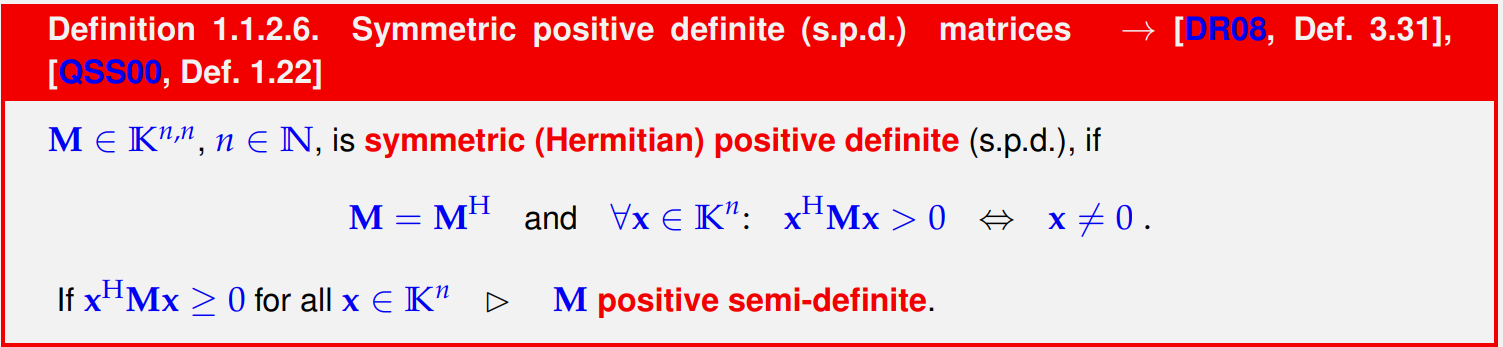
\includegraphics[width=1.0\linewidth]{PostiveSemiDefinite.png}
\end{figure}


\paragraph{1. $\mathbf{Q}$ has orthonormal columns:} We can verify this in the following way
\begin{equation*}
    \mathbf{Q}^{\mathsf{T}}\mathbf{Q} = \left(\mathbf{U}\mathbf{V}^{\mathsf{T}}\right)^{\mathsf{T}}\left(\mathbf{U}\mathbf{V}^{\mathsf{T}}\right) = \left(\mathbf{V}^{\mathsf{T}}\right)^{\mathsf{T}}\mathbf{U}^{\mathsf{T}}\mathbf{U}\mathbf{V}^{\mathsf{T}} = \mathbf{V}\underbrace{\mathbf{U}^{\mathsf{T}}\mathbf{U}}_{= \mathbf{I}}\mathbf{V}^{\mathsf{T}} = \mathbf{V}\mathbf{V}^{\mathsf{T}} = \mathbf{I}
\end{equation*}
\paragraph{2. $\mathbf{M}$ is symmetric positive semi-definite: } We first verify that $\mathbf{M}$ is symmetric.
\begin{equation*}
    \left(\mathbf{V}\mathbf{\Sigma}\mathbf{V}^{\mathsf{T}} \right)^{\mathsf{T}} = \left(\mathbf{V}^{\mathsf{T}}\right)^{\mathsf{T}}\mathbf{\Sigma}^{\mathsf{T}}\mathbf{V}^{\mathsf{T}} = \mathbf{V}\mathbf{\Sigma}\mathbf{V}^{\mathsf{T}}
\end{equation*}
We must remember here that $\mathbf{\Sigma}$ is symmetric and the rules for transposing of products of matrices. Next we verify that $\mathbf{M}$ is positive semi-definite. We have for some arbitrary $\mathbf{x}\in \mathbb{R}^{n,n}$
\begin{equation*}
    \mathbf{x}^{\mathsf{T}}\mathbf{M}\mathbf{x} =\mathbf{x}^{\mathsf{T}}\mathbf{V}\mathbf{\Sigma}\mathbf{V}^{\mathsf{T}}\mathbf{x} = \left(\mathbf{V}^{\mathsf{T}}\mathbf{x}\right)^{\mathsf{T}}\mathbf{\Sigma}\mathbf{V}^{\mathsf{T}}\mathbf{x} =\mathbf{y}^{\mathsf{T}}\mathbf{\Sigma}\mathbf{y}  \overset{(1)}{\geq} 0
\end{equation*}
We know remember that $\mathbf{\Sigma}$ is itself positive semi-definite and thus we can do the step $(1)$, where $\mathbf{y} = \mathbf{V}^{\mathsf{T}}\mathbf{x}$. Hence our decomposition is correct and the theorem is proven.
\subsection*{3-12.b}
We are given the following class description of \verb|PolarDecomposition|.


\begin{figure}[!hbt]
    \centering
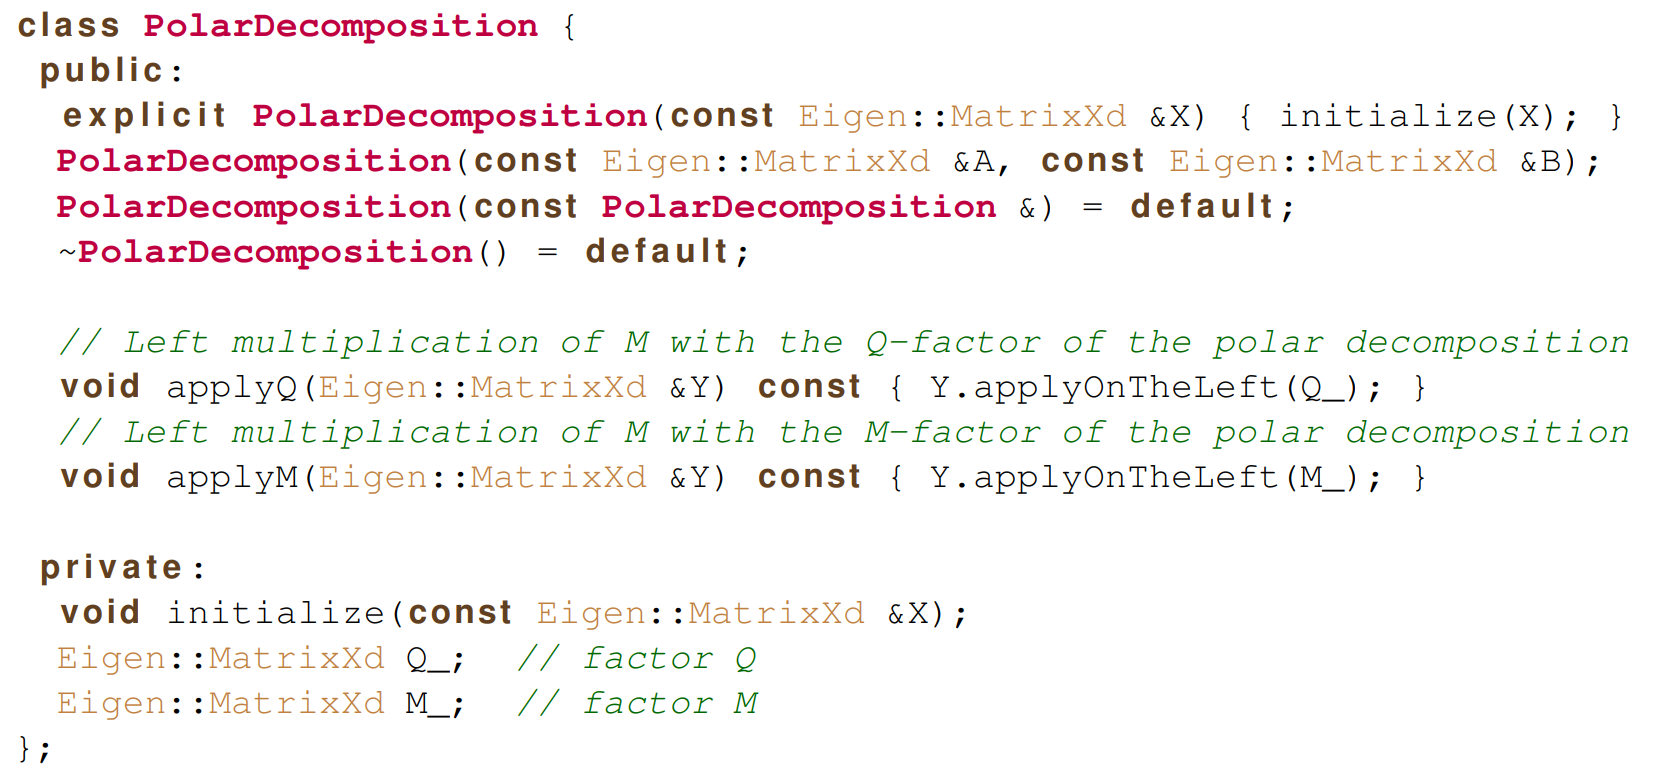
\includegraphics[width=1.0\linewidth]{PolarDecompositionClass.png}
\end{figure}
The second constructor computes the polar decomposition of $\mathbf{A}\mathbf{B}^{\mathsf{T}}$. We are tasked with determining the \textbf{minimial} asymptotic computational cost, that is, a \textbf{sharp lower bound} of asymptotic computational effort, for a call of the second constructor. A sharp lower bound can be given by the initialization of the memmbers \verb|Q_| and \verb|M_|. We have $\mathbf{Q}\in \mathbb{R}^{m,n}$ and $\mathbf{M}\in\mathbb{R}^{n,n}$. Hence accessing every entry and initializing it gives us a bound regardless of how the method is implemented.
\begin{equation*}
    \underbrace{\mathcal{O}\left(mn\right)}_{\text{Init. of }\mathbf{Q}} + \underbrace{\mathcal{O}\left(n^{2}\right)}_{\text{Init. of }\mathbf{M}} = \mathcal{O}\left(mn + n^{2}\right)
\end{equation*}
\subsection*{3-12.c}
We are tasked with implementing the method \verb|initialize| that takes a matrix \verb|X| as matrix and uses the construction discussed in 3-12.a to find $\mathbf{Q}$ and $\mathbf{M}$ according to Theorem 3.12.1. These should then be stored inside the members \verb|Q_| and \verb|M_|. We will once more use the lecture document as guide.
\begin{figure}[!hbt]
    \centering
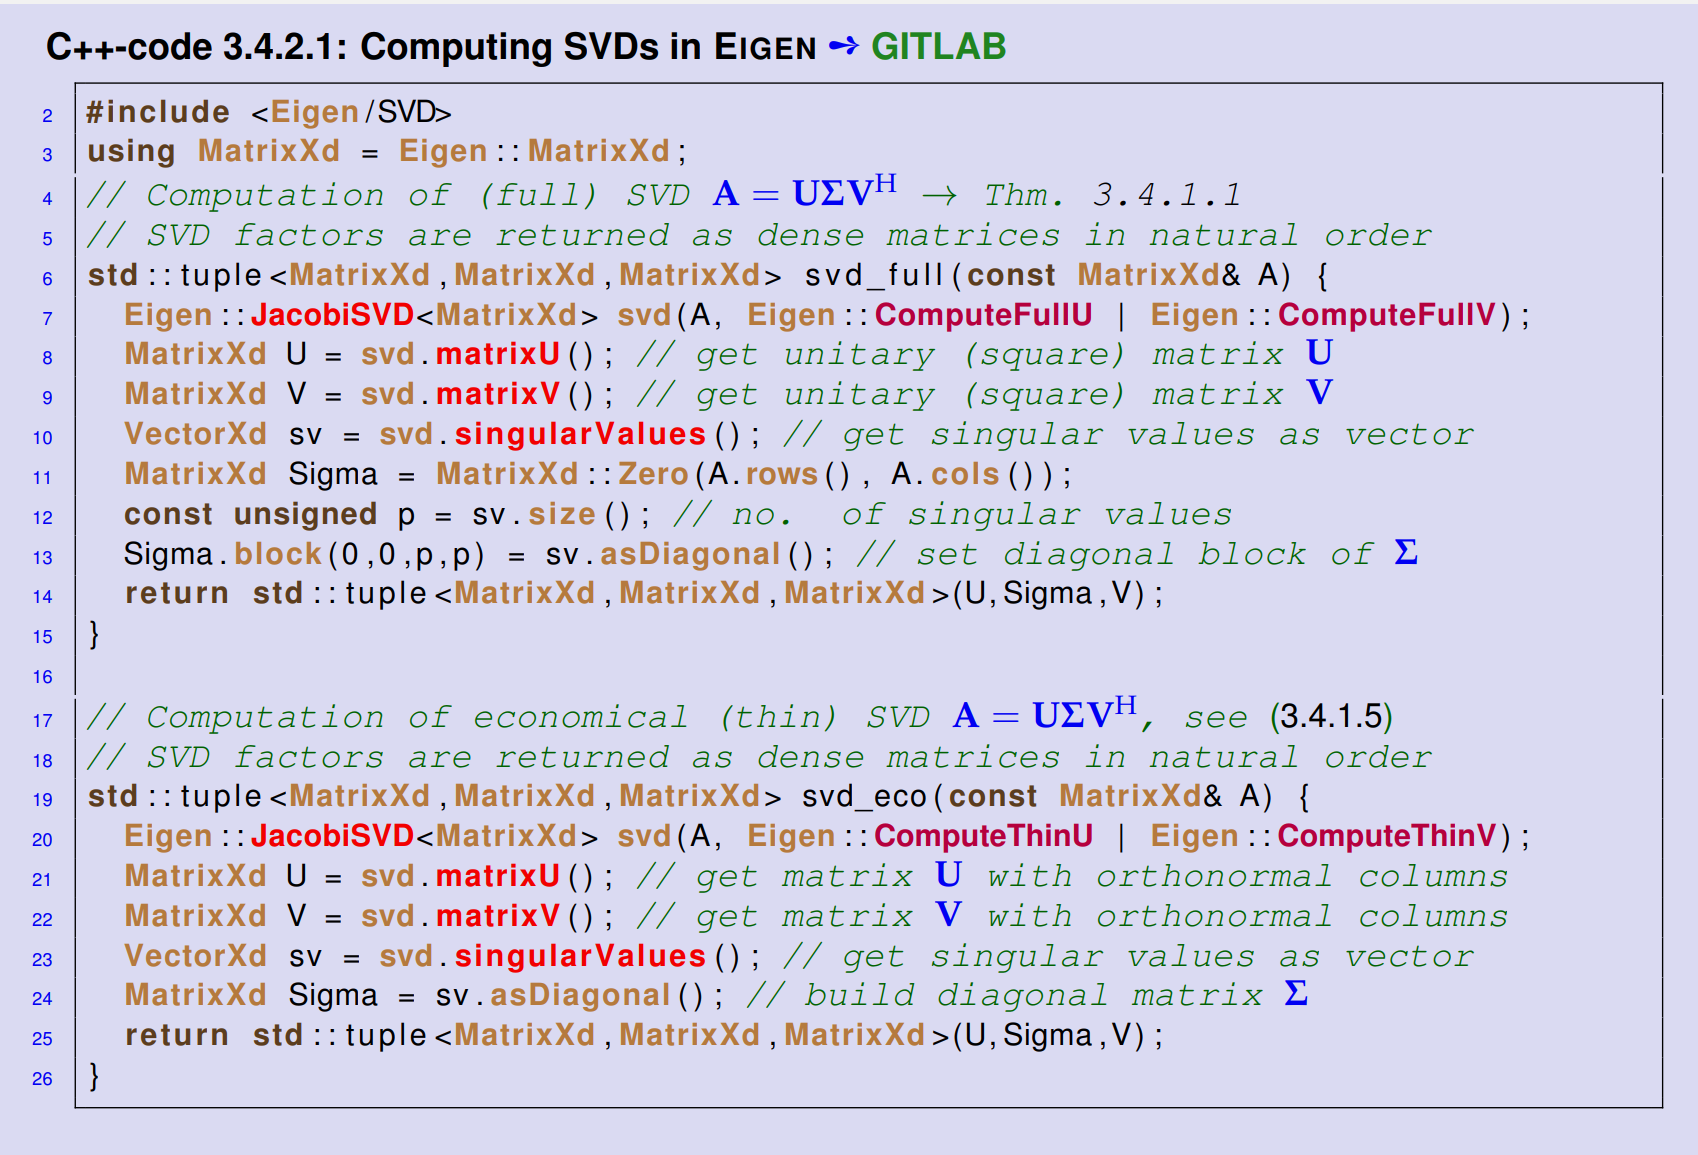
\includegraphics[width=1.0\linewidth]{JacobiSVD.png}
\end{figure}

\noindent This gives us the following code.
\begin{figure}[!hbt]
    \centering
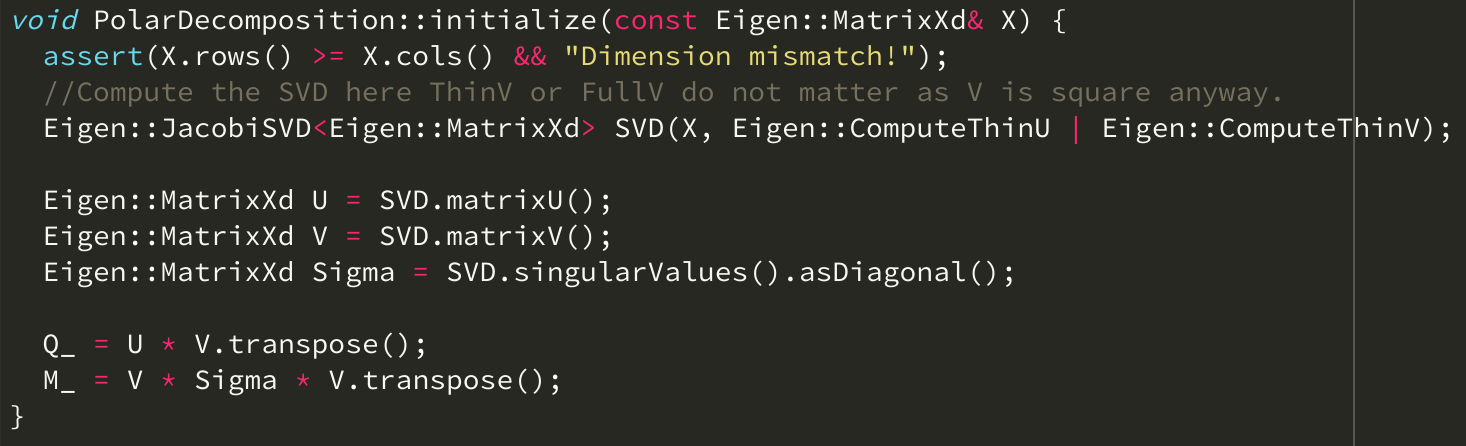
\includegraphics[width=1.0\linewidth]{3-12.c.png}
\end{figure}
\subsection*{3-12.d}
Now we are tasked with implementing the second constructor which should compute the polar decomposition for $\mathbf{A}\mathbf{B}^{\mathsf{T}}$, where $\mathbf{A}\in \mathbb{R}^{m,k}$ and $\mathbf{B}\in \mathbb{R}^{n,k}$ and $k \leq n \leq m$  is small and fixed. Our code should have \textbf{optimal complexity} with respect to $m$ and $n$. Let us first consider the structure, multiplying the matrices and taking the QR (using the hint) of that would not be a valid option as it would remove $k$ from the computational complexity of the computation of the QR, we do not want this. Let us thus consider taking the QR of both matrices individually and seeing if we can combine them to form a polar decomposition. We write
\begin{align*}
    \mathbf{A} &= \mathbf{Q}_{A}\mathbf{\tilde{R}}_{A} \\
    \mathbf{B} &= \mathbf{Q}_{B}\mathbf{\tilde{R}}_{B}
\end{align*}
The full QR-decomposition gives us
\begin{figure}[!hbt]
    \centering
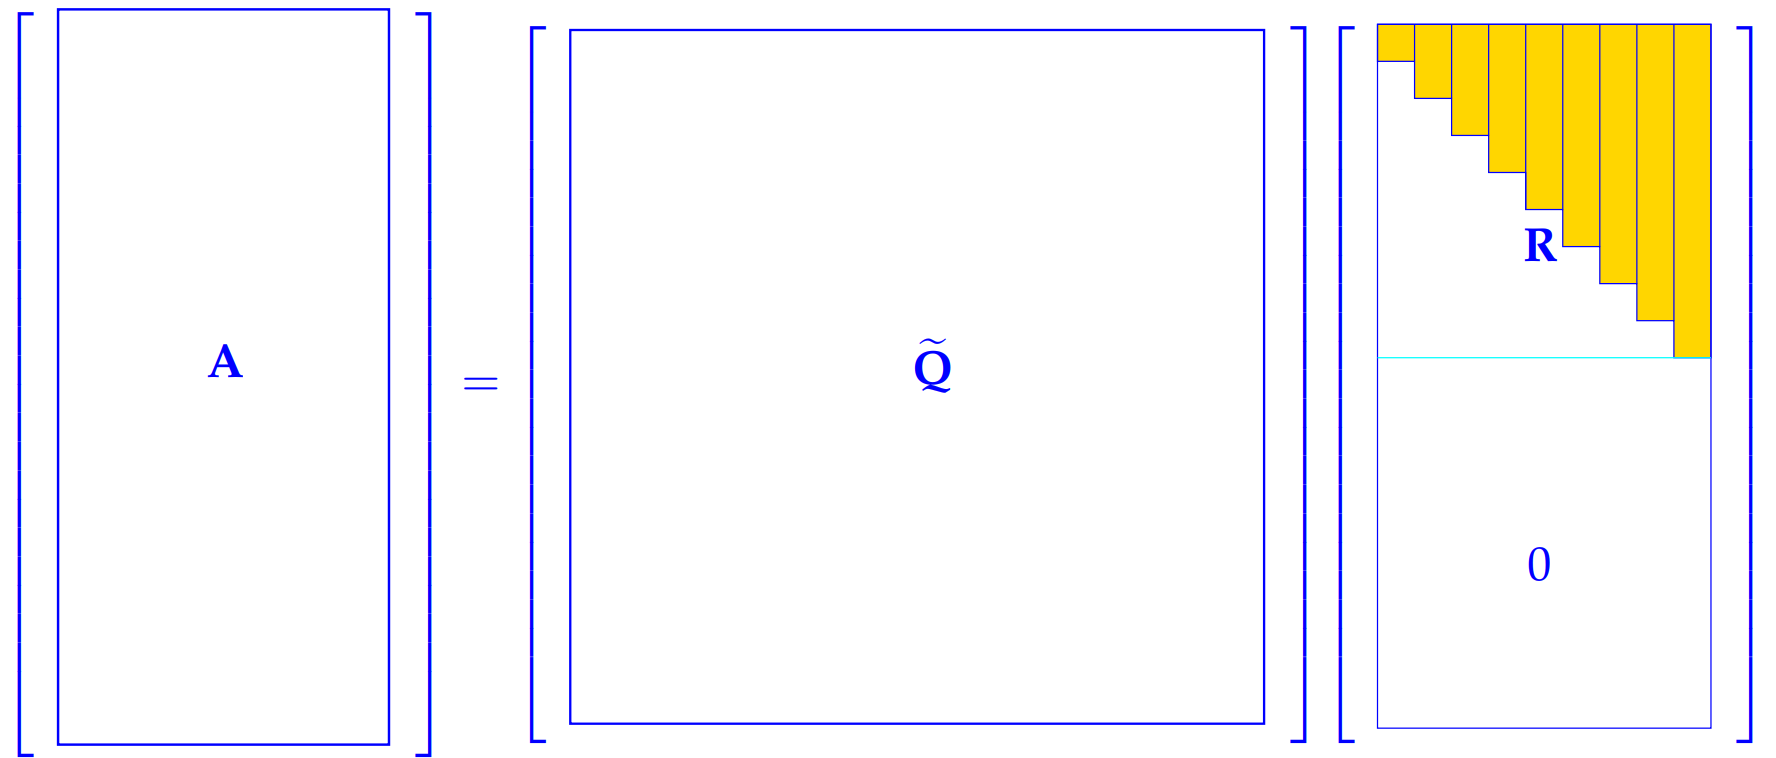
\includegraphics[width=1.0\linewidth]{QRFullDecomposition.png}
\end{figure} \\
We have 
\begin{align*}
    \mathbf{A}\in \mathbb{R}^{m,k} \, &: \: \mathbf{Q}_{A} \in \mathbb{R}^{m,m} \: \mathbf{\tilde{R}}_{A} \in \mathbb{R}^{m,k} \\
    \mathbf{B}\in \mathbb{R}^{n,k} \, &: \: \mathbf{Q}_{B} \in \mathbb{R}^{n,n} \:\: \,\mathbf{\tilde{R}}_{B} \in \mathbb{R}^{n,k}
\end{align*}
where we have 
\begin{equation*}
    \mathbf{\tilde{R}}_{A} = \begin{bmatrix}
    \mathbf{R}_{A}\\
    \mathbf{O}
    \end{bmatrix} \quad \mathbf{\tilde{R}}_{B} = \begin{bmatrix}
    \mathbf{R}_{B}\\
    \mathbf{O}
    \end{bmatrix}
\end{equation*}
Both $\mathbf{Q}$ matrices have orthonormal columns, and both the $\mathbf{R}$ matrices are upper triangular. We now derive from this the SVD of $\mathbf{A}\mathbf{B}^{\mathsf{T}}$
\begin{align*}
    \mathbf{X} = \mathbf{A}\mathbf{B}^{\mathsf{T}} &= \mathbf{Q}_{A}\begin{bmatrix}
    \mathbf{R}_{A}\\
    \mathbf{O}
    \end{bmatrix}
    \begin{bmatrix}
    \mathbf{R}_{B} & \mathbf{O}
    \end{bmatrix}\mathbf{Q}_{B}^{\mathsf{T}} \\
    &= \mathbf{Q}_{A}
    \begin{bmatrix}
        \mathbf{R}_{A}\mathbf{R}_{B} & \mathbf{O} \\
        \mathbf{O} & \mathbf{O}
    \end{bmatrix}
    \mathbf{Q}_{B}^{\tr} \\
\end{align*}
at this point we cannot continue further and thus computing the SVD of one of the terms involved seems sensible, seeing as both $\mathbf{Q}_{A}$ and $\mathbf{Q}_{B}$ have orthonormal columns we might need them later on, so we will take the SVD of the term $\mathbf{R}_{A}\mathbf{R}_{B}$. 
\begin{equation*}
  \mathbf{R}_{A}\mathbf{R}_{B} = \mathbf{\tilde{U}}\mathbf{\tilde{\Sigma}}\mathbf{\tilde{V}}^{\tr}  
\end{equation*}
We can continue the computation from above now.
\begin{align*}
    \mathbf{Q}_{A}
    \begin{bmatrix}
        \mathbf{R}_{A}\mathbf{R}_{B} & \mathbf{O} \\
        \mathbf{O} & \mathbf{O}
    \end{bmatrix}
    \mathbf{Q}_{B}^{\tr} &= \mathbf{Q}_{A}
    \begin{bmatrix}
        \mathbf{\tilde{U}}\mathbf{\tilde{\Sigma}}\mathbf{\tilde{V}}^{\tr}   & \mathbf{O} \\
        \mathbf{O} & \mathbf{O}
    \end{bmatrix}
    \mathbf{Q}_{B}^{\tr} \\
    &= \underbrace{\mathbf{Q}_{A} \begin{bmatrix}
        \mathbf{\tilde{U}} & \mathbf{O} \\
        \mathbf{O} & \mathbf{I} \\
        \mathbf{O} & \mathbf{O}
    \end{bmatrix}}_{=:\mathbf{U}}
    \underbrace{\begin{bmatrix}
        \mathbf{\tilde{\Sigma}} & \mathbf{O} \\
        \mathbf{O} & \mathbf{O}
    \end{bmatrix}}_{=:\mathbf{\Sigma}}
    \underbrace{\begin{bmatrix}
        \mathbf{\tilde{V}}^{\tr} & \mathbf{O} \\
        \mathbf{O} & \mathbf{I}
    \end{bmatrix}\mathbf{Q}_{B}^{\tr}}_{=:\mathbf{V}^{\tr}}
\end{align*}
I thank Cédric Laubacher for this answer as I really did not understand what was done until seeing their answer on the exam collection. The padding is done for the multiplications to be compatible and the insertion of identity matrices is done to ensure that the columns are orthonormal. We can immediately see that $\mathbf{\Sigma}$ is diagonal with non-negative entries, this follows from the SVD od $\mathbf{R}_{A}\mathbf{R}_{B}$. Now we apply that the product of two matrices with orthonormal columns also has orthonormal columns. Let thus $\mathbf{G}$ and $\mathbf{H}$ be two matrices with orthonormal columns, we have $\mathbf{G}^{\tr}\mathbf{G} = \mathbf{I}$ and $\mathbf{H}^{\tr}\mathbf{H} = \mathbf{I}$ and thus
\begin{equation*}
    \left(\mathbf{G}\mathbf{H}\right)^{\tr}\mathbf{G}\mathbf{H} = \mathbf{H}^{\tr}\underbrace{\mathbf{G}^{\tr}\mathbf{G}}_{= \mathbf{I}}\mathbf{H} = \mathbf{H}^{\tr}\mathbf{H} = \mathbf{I}
\end{equation*}
hence both $\mathbf{U}$ and $\mathbf{V}$ as defined above have orthonormal columns. We then define $\mathbf{Q}$ and $\mathbf{M}$ as follows.
\begin{equation*}
    \mathbf{Q} = \mathbf{U}\mathbf{V}^{\tr} \in \mathbb{R}^{m,n} \quad \mathbf{M} := \mathbf{V}\begin{bmatrix}
        \mathbf{\tilde{\Sigma}} &\mathbf{O} \\
        \mathbf{O} & \mathbf{O}
    \end{bmatrix}\mathbf{V}^{\tr}
\end{equation*}
Here we use the same structure as in 3-12.a again. We have
\begin{align*}
    \mathbf{Q}\mathbf{M} = \mathbf{U}\underbrace{\mathbf{V}^{\tr} \mathbf{V}}_{=\mathbf{I}}\begin{bmatrix}
        \mathbf{\tilde{\Sigma}} &\mathbf{O} \\
        \mathbf{O} & \mathbf{O}
    \end{bmatrix}\mathbf{V}^{\tr} &= \mathbf{U}\begin{bmatrix}
        \mathbf{\tilde{\Sigma}} &\mathbf{O} \\
        \mathbf{O} & \mathbf{O}
    \end{bmatrix}\mathbf{V}^{\tr} \\
    &=\mathbf{Q}_{A} \begin{bmatrix}
        \mathbf{\tilde{U}} & \mathbf{O} \\
        \mathbf{O} & \mathbf{I} \\
        \mathbf{O} & \mathbf{O}
    \end{bmatrix}\begin{bmatrix}
        \mathbf{\tilde{\Sigma}} & \mathbf{O} \\
        \mathbf{O} & \mathbf{O}
    \end{bmatrix}\begin{bmatrix}
        \mathbf{\tilde{V}}^{\tr} & \mathbf{O} \\
        \mathbf{O} & \mathbf{I}
    \end{bmatrix}\mathbf{Q}_{b}^{\tr} \\
    &=  \mathbf{Q}_{A}
    \begin{bmatrix}
        \mathbf{\tilde{U}}\mathbf{\tilde{\Sigma}}\mathbf{\tilde{V}}^{\tr}   & \mathbf{O} \\
        \mathbf{O} & \mathbf{O}
    \end{bmatrix}
    \mathbf{Q}_{B}^{\tr} \\
    &=  \mathbf{Q}_{A}
    \begin{bmatrix}
        \mathbf{R}_{A}\mathbf{R}_{B} & \mathbf{O} \\
        \mathbf{O} & \mathbf{O}
    \end{bmatrix}
    \mathbf{Q}_{B}^{\tr} \\
    &= \mathbf{Q}_{A}\begin{bmatrix}
    \mathbf{R}_{A}\\
    \mathbf{O}
    \end{bmatrix}
    \begin{bmatrix}
    \mathbf{R}_{B} & \mathbf{O}
    \end{bmatrix}\mathbf{Q}_{B}^{\mathsf{T}} \\
    &= \mathbf{A}\mathbf{B}^{\tr} \\
    &= \mathbf{X}
\end{align*}

\pagebreak

\noindent So $\mathbf{Q}$ and $\mathbf{M}$ as a product are $\mathbf{X}$. Now we need to check that the proposed polar decomposition is correct. 

\paragraph{$\mathbf{Q}$ has orthonormal columns:} We have $\mathbf{Q} = \mathbf{U}\mathbf{V}^{\tr}$ and thus
\begin{equation*}
    \mathbf{Q}^{\tr}\mathbf{Q} = \mathbf{V}\underbrace{\mathbf{U}^{\tr}\mathbf{U}}_{= \mathbf{I}}\mathbf{V}^{\tr} = \mathbf{V}\mathbf{V}^{\tr} = \mathbf{I}
\end{equation*}
hence $\mathbf{Q}$ has orthonormal columns.
\paragraph{$\mathbf{M}$ is symmetric:} We can check this as follows.
\begin{equation*}
    \mathbf{M}^{\tr} = \left(\mathbf{V}\begin{bmatrix}
        \mathbf{\tilde{\Sigma}} &\mathbf{O} \\
        \mathbf{O} & \mathbf{O}
    \end{bmatrix}\mathbf{V}^{\tr}\right)^{\tr} = \left(\mathbf{V}^{\tr}\right)^{\tr}\begin{bmatrix}
        \mathbf{\tilde{\Sigma}} &\mathbf{O} \\
        \mathbf{O} & \mathbf{O}
    \end{bmatrix}^{\tr}\mathbf{V}^{\tr} 
    = \mathbf{V}\begin{bmatrix}
        \mathbf{\tilde{\Sigma}} &\mathbf{O} \\
        \mathbf{O} & \mathbf{O}
    \end{bmatrix}^{\tr}\mathbf{V}^{\tr}
\end{equation*}
Because $\mathbf{\tilde{\Sigma}}$ is diagonal and thus symmetric and all other entries of the block matrix above ar zero, we can see that itself it must also be symmetric, this leads to
\begin{equation*}
    \mathbf{V}\begin{bmatrix}
        \mathbf{\tilde{\Sigma}} &\mathbf{O} \\
        \mathbf{O} & \mathbf{O}
    \end{bmatrix}^{\tr}\mathbf{V}^{\tr} = \mathbf{V}\begin{bmatrix}
        \mathbf{\tilde{\Sigma}} &\mathbf{O} \\
        \mathbf{O} & \mathbf{O}
    \end{bmatrix}\mathbf{V}^{\tr} = \mathbf{M}
\end{equation*}
hence $\mathbf{M}$ is symmetric.
\paragraph{$\mathbf{M}$ is positive semi-definite:} Let $\mathbf{x}\in\mathbb{R}^{n}$ then we have
\begin{equation*}
\mathbf{x}^{\tr}\mathbf{M}\mathbf{x} = 
   \mathbf{x} ^{\tr}\mathbf{V}\begin{bmatrix}
        \mathbf{\tilde{\Sigma}} &\mathbf{O} \\
        \mathbf{O} & \mathbf{O}
    \end{bmatrix}\mathbf{V}^{\tr} \mathbf{x} = \left(\mathbf{V}^{\tr}\mathbf{x}\right)^{\tr}\begin{bmatrix}
        \mathbf{\tilde{\Sigma}} &\mathbf{O} \\
        \mathbf{O} & \mathbf{O}
    \end{bmatrix} \left(\mathbf{V}^{\tr}\mathbf{x}\right) = \mathbf{y}^{\tr}\underbrace{\begin{bmatrix}
        \mathbf{\tilde{\Sigma}} &\mathbf{O} \\
        \mathbf{O} & \mathbf{O}
    \end{bmatrix}}_{=: \mathbf{\Sigma}}\mathbf{y}
\end{equation*}
we can see that $\mathbf{\Sigma}$ is diagonal with only non-negative diagonal entries and thus positive semi-definite. From this it follows with $\mathbf{y} = \mathbf{V}^{\tr}\mathbf{x}$ that the matrix $\mathbf{M}$ must also be positive semi-definite. 

\paragraph{Computation of $\mathbf{Q}$:} We have that $\mathbf{Q}$ is computed in the following form 
\begin{equation*}
    \mathbf{Q} = \mathbf{U}\mathbf{V}^{\tr} = \underbrace{\mathbf{Q}_{A}}_{\in \mathbb{R}^{m,m}} \underbrace{\begin{bmatrix}
        \mathbf{\tilde{U}} & \mathbf{O} \\
        \mathbf{O} & \mathbf{I} \\
        \mathbf{O} & \mathbf{O}
    \end{bmatrix}}_{\in \mathbb{R}^{m,n}}\underbrace{\begin{bmatrix}
        \mathbf{\tilde{V}}^{\tr} & \mathbf{O} \\
        \mathbf{O} & \mathbf{I}
    \end{bmatrix}}_{\in \mathbb{R}^{n,n}}\underbrace{\mathbf{Q}_{B}^{\tr}}_{\in \mathbb{R}^{n,n}}
\end{equation*}
for the sake of efficiency we must now be careful in what order we make these matrix multiplications. Multiplying the middle blocks first as the block matrix multiplication allows for only the product $\mathbf{\tilde{U}}\mathbf{\tilde{V}}^{\tr}$ to be computed where $\mathbf{\tilde{U}}, \mathbf{\tilde{V}}^{\tr} \in \mathbb{R}^{k,k}$ and hence this does not add to the cost as $k$ is constant and we compute the cost in view of $n$ and $m$. This gives us
\begin{equation*}
    \mathbf{Q}_{A}\begin{bmatrix}
        \mathbf{\tilde{U}} & \mathbf{O} \\
        \mathbf{O} & \mathbf{I} \\
        \mathbf{O} & \mathbf{O}
    \end{bmatrix}\begin{bmatrix}
        \mathbf{\tilde{V}}^{\tr} & \mathbf{O} \\
        \mathbf{O} & \mathbf{I}
    \end{bmatrix}\mathbf{Q}_{B}^{\tr} = \mathbf{Q}_{A}
    \begin{bmatrix}
      \mathbf{\tilde{U}}\mathbf{\tilde{V}}^{\tr}  & \mathbf{O} \\
      \mathbf{O} & \mathbf{I} \\
      \mathbf{O} & \mathbf{O}
      
    \end{bmatrix}
    \mathbf{Q}_{B}^{\tr}
\end{equation*}
This leads to the final computation order
\begin{equation*}
    \mathbf{Q} = \left(\mathbf{Q}_{B}\left(\mathbf{Q}_{A}\begin{bmatrix}
        \mathbf{\tilde{U}}\mathbf{\tilde{V}}^{\tr}  & \mathbf{O} \\
      \mathbf{O} & \mathbf{I} \\
      \mathbf{O} & \mathbf{O}
      
    \end{bmatrix}\right)^{\tr}\right)^{\tr}
\end{equation*}
beware that the transposition is what allows us to compute this in the order specified above.
\paragraph{Computation of $\mathbf{M}$: } We have the following computation for $\mathbf{M}$
\begin{equation*}
    \mathbf{M} = \mathbf{V}\begin{bmatrix}
        \mathbf{\tilde{\Sigma}} &\mathbf{O} \\
        \mathbf{O} & \mathbf{O}
    \end{bmatrix}^{\tr}\mathbf{V}^{\tr} = 
    \underbrace{\mathbf{Q}_{B}}_{\in \mathbb{R}^{n,n}}
    \underbrace{\begin{bmatrix}
        \mathbf{\tilde{V}} & \mathbf{O} \\
        \mathbf{O} & \mathbf{I}
    \end{bmatrix}}_{\in \mathbb{R}^{n,n}}\underbrace{\begin{bmatrix}
        \mathbf{\tilde{\Sigma}} &\mathbf{O} \\
        \mathbf{O} & \mathbf{O}
    \end{bmatrix}^{\tr}}_{\in \mathbb{R}^{n,n}}\underbrace{\begin{bmatrix}
        \mathbf{\tilde{V}}^{\tr} & \mathbf{O} \\
        \mathbf{O} & \mathbf{I}
    \end{bmatrix}}_{\in \mathbb{R}^{n,n}}\underbrace{\mathbf{Q}_{B}^{\tr}}_{\in \mathbb{R}^{n,n}}
\end{equation*}
here we again first multiply the block which again does not amount any asymptotic cost besides a constant factor $k$ which gives us the final computation order for $\mathbf{M}$.
\begin{equation*}
    \mathbf{M} = \left(\mathbf{Q}_{B}\left(\mathbf{Q}_{B}\begin{bmatrix}
        \mathbf{\tilde{V}}\mathbf{\tilde{\Sigma}}\mathbf{\tilde{V}}^{\tr}   & \mathbf{O} \\
        \mathbf{O} & \mathbf{O}
    \end{bmatrix}\right)^{\tr}\right)^{\tr}
\end{equation*}
\paragraph{Computational cost:} The SVD of $\mathbf{R}_{A}\mathbf{R}_{B} \in \mathbb{R}^{k,k}$ can be diregarded in terms of $m$ and $n$, what matters the most is the multiplication with $\mathbf{Q}_{A}$ and $\mathbf{Q}_{B}$ in the construction for $\mathbf{Q}$ and $\mathbf{M}$. In the computation of $\mathbf{Q}$ we multiply once with $\mathbf{Q}_{A}$ giving us the cost of $\mathcal{O}\left(mn\right)$ (multiplying with "vector" of length $n$) and then multiply the result with $\mathbf{Q}_{B}$ which us $\mathcal{O}\left(n^{2}\right)$ and overall $\mathcal{O}\left(mn + n^{2}\right)$. A similar argument leads to the computational cost for the construction of $\mathbf{M}$ being $\mathcal{O}\left(n^{2}\right)$ and thus overall we get $\mathcal{O}\left(mn + n^{2}\right)$ which is the postulated lower bound for the computation. 

\paragraph{The code:} All that is left is to implement this. We first take a look at the following code as a guide on how to use the economical QR decomposition in Eigen found as part of Code 3.3.4.1 in the lecture document.

\begin{figure}[!hbt]
    \centering
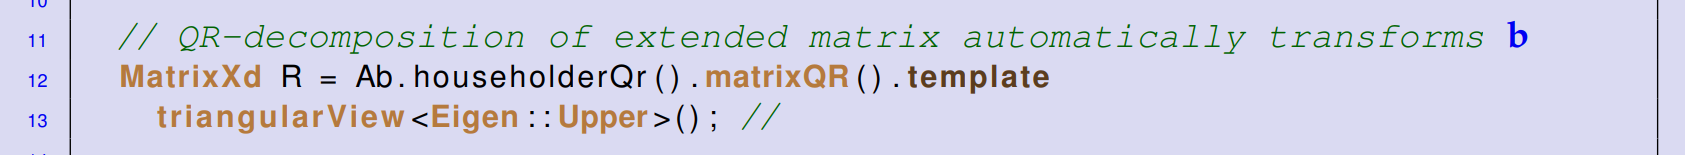
\includegraphics[width=1.0\linewidth]{QRThinEigen.png}
\end{figure}
The block assignments that are made in the following code come from the following structure.
\begin{equation*}
    \begin{bmatrix}
        \mathbf{\tilde{U}}\mathbf{\tilde{V}}^{\tr}  & \mathbf{O} \\
      \mathbf{O} & \mathbf{I} \\
      \mathbf{O} & \mathbf{O}
      
    \end{bmatrix} =
    \begin{bmatrix}
        \mathbf{\tilde{U}}\mathbf{\tilde{V}}^{\tr}  & \mathbf{O}_{k,n-k} \\
      \mathbf{O}_{n-k,k} & \mathbf{I}_{n-k} \\
      \mathbf{O}_{m-n,k} & \mathbf{O}_{m-n,n-k}
      
    \end{bmatrix} \quad 
    \begin{bmatrix}
        \mathbf{\tilde{V}}\mathbf{\tilde{\Sigma}}\mathbf{\tilde{V}}^{\tr}   & \mathbf{O} \\
        \mathbf{O} & \mathbf{O}
    \end{bmatrix}=\begin{bmatrix}
        \mathbf{\tilde{V}}\mathbf{\tilde{\Sigma}}\mathbf{\tilde{V}}^{\tr}   & \mathbf{O}_{k, n-k} \\
        \mathbf{O}_{n-k,k} & \mathbf{O}_{n-k,n-k}
    \end{bmatrix} 
\end{equation*}

\pagebreak

\noindent This then gives us the following code.
\begin{figure}[!hbt]
    \centering
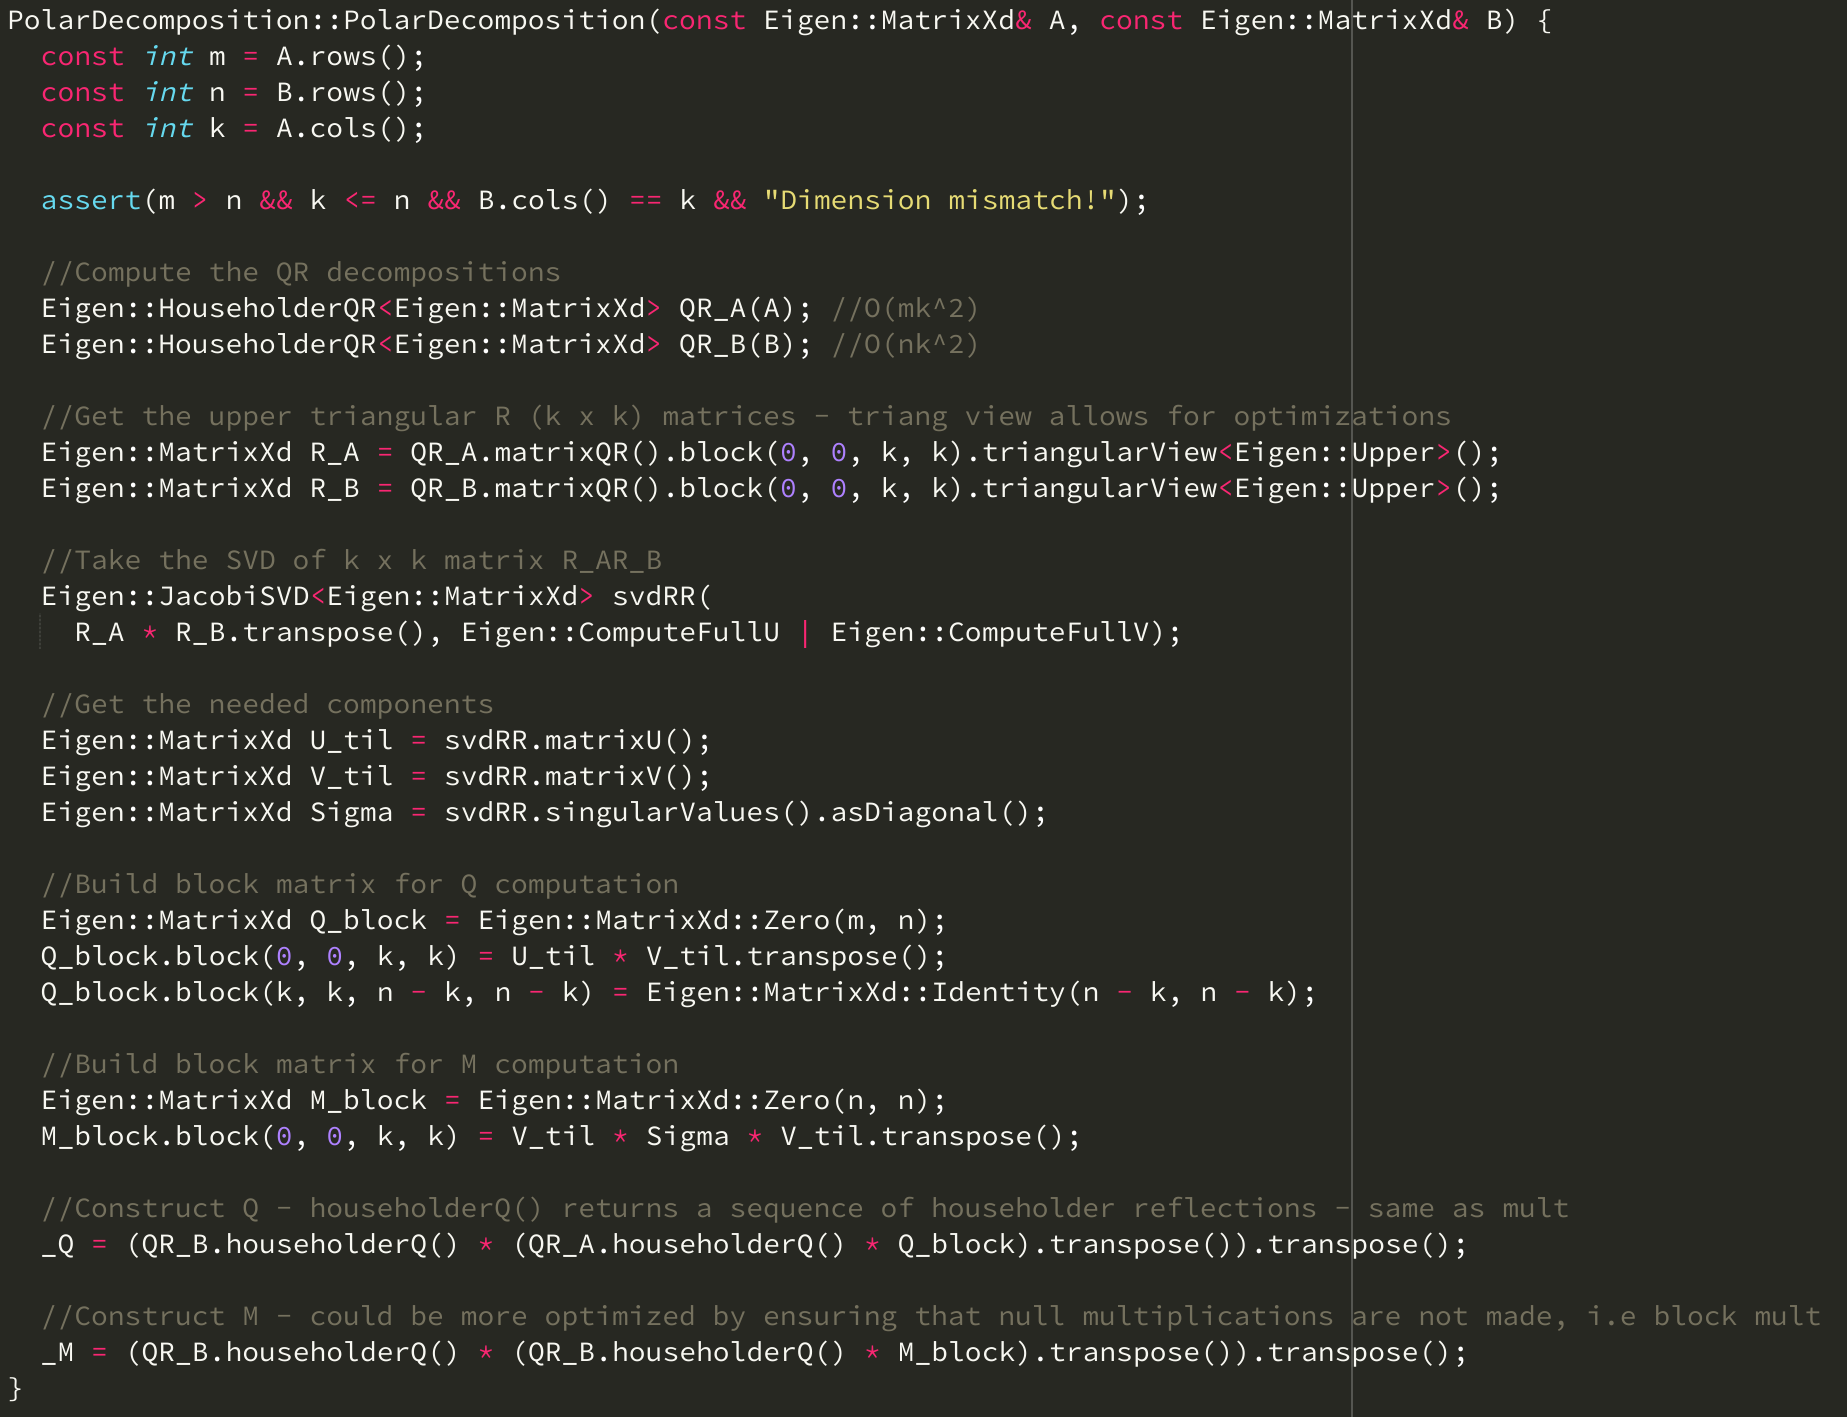
\includegraphics[width=1.0\linewidth]{3-12.d.png}
\end{figure}
\end{document}
